%==================================================================================================
% Workaround for XeTeX compilation with the 'fontspec' and 'europecv' packages
%==================================================================================================

% Pretend that the 'inputenc' package was loaded with the 'utf8x' option

\makeatletter
    \@namedef{ver@inputenc.sty}{}
    \@namedef{opt@inputenc.sty}{utf8x}
\makeatother

\expandafter\let\csname ver@inputenc.sty \endcsname\relax

% Neutralize the '\inputencoding' command used by the 'europecv' package

\providecommand{\inputencoding}[1]{}


%==================================================================================================
% LaTeX markup to typeset a Curriculm Vitae using the 'europecv' package
%==================================================================================================

\documentclass[a4paper,english,totpages]{europecv}

\usepackage[top=1.5cm, bottom=1.5cm, left=1.5cm, right=1.5cm]{geometry}
\usepackage[english]{babel}
\usepackage[T1]{fontenc}
\usepackage{fontspec}
\usepackage{enumitem}
\usepackage{graphicx}
\usepackage{hyperref}
\usepackage{xcolor}



%--------------------------------------------------------------------------------------------------
% General configuration for the loaded packages
%--------------------------------------------------------------------------------------------------

\defaultfontfeatures{Ligatures=TeX}
\setmainfont{Arial}

\setlist{
    leftmargin=*,
    nolistsep,
    itemsep=2pt
}

\definecolor{RoyalBlue}{RGB}{65, 105, 225}

\hypersetup{
    bookmarksopen=false,
    colorlinks=true,
    urlcolor=RoyalBlue,
    pdfpagemode=UseNone,
    pdfstartview={FitH},
    pdfdisplaydoctitle=true,
    pdfinfo={
        Title={Tiago Fael Matos' Curriculm Vitae},
        Author={Tiago Fael Matos},
        Subject={Curriculum Vitae typesetted in LaTeX based on the Europass model}
    },
    pdfcreator={XeLaTeX}
}

% Reduce the amount of lookahead to avoid clearing the footer on wrong pages

\setcounter{LTchunksize}{1}

%--------------------------------------------------------------------------------------------------
% Allow changes to internal LaTeX macros outside packages/classes
%--------------------------------------------------------------------------------------------------

\makeatletter

    % Improve document title style

    \renewcommand*\ecvtitle{\ecv@utf{\Large\textbf{Curriculum Vitae}\\[5pt]\Large\textbf{Europass}}}

    % Improve 'europecv' language table and string styles

    \def\ecv@mothertonguekey{\ecv@utf{\normalsize Mother Tongue}}
    \def\ecv@assesskey{\ecv@utf{\normalsize Self-Assessment}}
    \def\ecv@levelkey{\ecv@utf{\normalsize European Level}}
    \def\ecv@listenkey{\vspace{2pt}\ecv@utf{\scriptsize Listening}}
    \def\ecv@readkey{\vspace{2pt}\ecv@utf{\scriptsize Reading}}
    \def\ecv@interactkey{\vspace{2pt}\ecv@utf{\scriptsize Spoken Interaction}}
    \def\ecv@productkey{\vspace{2pt}\ecv@utf{\scriptsize Spoken Production}}
    \def\ecv@cefbasickey{\ecv@utf{\scriptsize Basic User}}
    \def\ecv@cefindepkey{\ecv@utf{{\scriptsize Independent User}}}
    \def\ecv@cefprofkey{\ecv@utf{\scriptsize Proficient User}}
    \def\ecv@langfooterkey{\ecv@utf{\href{http://europass.cedefop.europa.eu/en/resources/european-language-levels-cefr}{Common European Framework of Reference (CEF) Level}}}

    \renewcommand*\ecvCEF[2]{
        \begin{tabular}{@{}>{\footnotesize}m{.2\ecv@langparwidth}@{\hspace{1mm}}>{\footnotesize\centering}m{.74\ecv@langparwidth}@{}}
            #1 & #2\tabularnewline
        \end{tabular}
    }

    % Change lists bullet style to a black dot

    \renewcommand{\labelitemi}{$\bullet$}

    % Add a blue underline to URL links

    \Hy@AtBeginDocument{
        \def\@urlbordercolor{0.06 0.3 0.55}
        \def\@pdfborderstyle{0}
    }

    % Disable the total pages number link to the last page

    \def\ecv@totpages{~/~\ref*{TotPages}}

\makeatother

%--------------------------------------------------------------------------------------------------
% New commands to simplify the CV content markup
%--------------------------------------------------------------------------------------------------

\newcommand{\ccvsection}[2]{\pdfbookmark{#2}{#1}\ecvsection{#2}}
\newcommand{\ccvitem}[2]{\ecvitem[5pt]{#1}{#2}}

\newcommand{\ccvattachment}[4][10pt]{\pdfbookmark{#3}{attachment#2}{\large\par\textbf{#3}}\vspace{#1} & {\par#4}\tabularnewline\nopagebreak}

\newcommand{\weblink}[1]{\href{#1}{#1}}
\newcommand{\maillink}[1]{\href{mailto:#1}{#1}}

%--------------------------------------------------------------------------------------------------
% The beginning of the actual CV document
%--------------------------------------------------------------------------------------------------

\begin{document}

    % Generic Europass CV information

    \ecvfootername{Tiago Fael Matos}
    \ecvfootnote{To connect with me on LinkedIn, please visit:\newline
        \weblink{http://www.linkedin.com/in/ktachyon}}

    % Decrease the total number of pages by the amount of appendix pages

    \addtocounter{TotPages}{-2}

    % The beginning of the Europass CV content

    \begin{europecv}

        % Top left profile photo

        & \ecvspace{-2.2cm} \raggedleft
        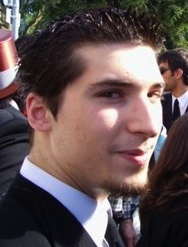
\includegraphics[width=3.5cm]{graphics/photo}
        \ecvspace{-2.2cm} \tabularnewline

        % Personal Information

        \ccvsection{personal}{Personal Information}

        \ccvitem{First Names / Surnames}{\large\textbf{Tiago Fael Gonçalves de Matos}}
        \InputIfFileExists{includes/sensible-en}{}{
            \ccvitem{Address}{\textit{(not shown due to privacy protection)}}
            \ccvitem{Mobile}{\textit{(not shown due to privacy protection)}}
            \ccvitem{Email}{\textit{(not shown due to privacy protection)}}
        }
        \ccvitem{Twitter}{\weblink{http://twitter.com/KTachyon}}
        \ccvitem{Nationality}{Portuguese}
        \ccvitem{Date of Birth}{16$^{th}$ September, 1985}
        \ccvitem{Gender}{Male}

        % Occupational Field

        \tabularnewline
        \ccvitem{\large\textbf{Occupational Field}}{\large\textbf{Software Engineering}}

        % Work Experience

        \ccvsection{work}{Work Experience}

        \ccvitem{Dates}{October 2014 $\longrightarrow$ now}
        \ccvitem{Occupation or Position Held}{\textbf{iOS Software Engineer, Fullstack Software Engineer}}
        \ccvitem{Main Activities and Responsibilities}{
            \begin{itemize}
                \item Development and optimization of components for the JiTT app (\weblink{https://itunes.apple.com/artist/iclio/id418757745});
                \item Full integration of Viator into the JiTT app (UI, logic and API communication);
                \item Development of a NodeJS based REST API;
                \item Development of a Backbone-based web client for the aforementioned API;
            \end{itemize}
        }
        \ccvitem{Name and Address of Employer}{iClio (\weblink{http://www.iclio.net})}
        \ccvitem{Type of Business or Sector}{Digital Tourism, Content Platform}

        \tabularnewline

        \ccvitem{Dates}{December 2012 $\longrightarrow$ October 2014}
        \ccvitem{Occupation or Position Held}{\textbf{Software Engineer}}
        \ccvitem{Main Activities and Responsibilities}{
            \begin{itemize}
                \item Development of an Android app and web services for management of parking meters;
                \item Development of an e-learning web application platform;
                \item Development of a Backbone-based framework for faster single-page web application development;
                \item Development of a platform for building web-based interactive books;
                \item Development of iOS and Android apps for paying paid parking spaces;
                \item Development of an iOS app for counting the time spent inside geofences and with iBeacon support;
            \end{itemize}
        }
        \ccvitem{Name and Address of Employer}{Premium Minds (\weblink{http://www.premium-minds.com})}
        \ccvitem{Type of Business or Sector}{Web and Mobile Software Development}

        \tabularnewline

        \ccvitem{Dates}{December 2012 $\longrightarrow$ July 2012}
        \ccvitem{Occupation or Position Held}{\textbf{Software Engineer}}
        \ccvitem{Main Activities and Responsibilities}{
            \begin{itemize}
                \item Development of the iOS app for Limetree (\weblink{http://limetr.ee});
                \item Web frontend development and payment systems integration;
                \item Participated with Limetree in Ryan Academy's Propeller Venture Accelerator in Dublin.
            \end{itemize}
        }
        \ccvitem{Name and Address of Employer}{Limetree (\weblink{http://limetr.ee})}
        \ccvitem{Type of Business or Sector}{Web and Mobile Web Software Development}

        \tabularnewline

        \ccvitem{Dates}{September 2010 $\longrightarrow$ October 2012}
        \ccvitem{Occupation or Position Held}{\textbf{Systems Administrator and Software Engineer}}
        \ccvitem{Main Activities and Responsibilities}{
            \begin{itemize}
                \item Development and management of UCV (\weblink{http://ucv.uc.pt}) based on an open source, Pylons-based video platform called MediaCore;
                \item Development of both UCV mobile applications for iOS (\weblink{http://itunes.apple.com/pt/app/ucv/id516297795}) and Android (\weblink{https://play.google.com/store/apps/details?id=pt.uc.ucv});
                \item Development of some support (web based) platforms for University of Coimbra's presence in iTunes U (\weblink{http://www.uc.pt/itunesU/coleccoes});
                \item Configuration of several key systems that support University of Coimbra's presence in iTunes U, one of those a dual-controller SAN connected to two Mac Pro's to be used as main and failover/failback controllers;
                \item Development and management of Agenda7 (\weblink{http://agenda7.uc.pt});
                \item Consultant on the HPIP project (\weblink{http://hpip.org});
                \item Remote management/administration of a dozen servers with CentOS, Fedora Core and Mac OS X Server operating systems.
            \end{itemize}
        }
        \ccvitem{Name and Address of Employer}{University of Coimbra (\weblink{http://www.uc.pt})}
        \ccvitem{Type of Business or Sector}{Higher education institution}

        \tabularnewline

        \ccvitem{Dates}{January 2010 $\longrightarrow$ May 2011}
        \ccvitem{Occupation or Position Held}{\textbf{iOS Developer}}
        \ccvitem{Main Activities and Responsibilities}{Development of iOS applications for major sporting events, where I developed 3 iOS applications:
            \begin{itemize}
                \item 2010 FIFA World Cup (ZA2010);
                \item 2010 FIBA World Cup (TR2010);
                \item 2011 AFC Asian Cup (QA2011);
            \end{itemize}
        The apps were taken off the app store since they were no longer relevant.}
        \ccvitem{Name and Address of Employer}{MajorSportsEvents (\weblink{http://www.majorsportsevents.com})}
        \ccvitem{Type of Business or Sector}{Mobile Software Development}

        \tabularnewline

        \ccvitem{Dates}{July 2010 $\longrightarrow$ September 2010}
        \ccvitem{Occupation or Position Held}{\textbf{iOS Developer}}
        \ccvitem{Main Activities and Responsibilities}{Development of iOS applications and server-side services. Developed components for the JiTT application for iOS.}
        \ccvitem{Name and Address of Employer}{iClio Lda. (\weblink{http://www.iclio.net}, \weblink{http://www.justintimetourist.com})\newline IPN - Instituto Pedro Nunes\newline Rua Pedro Nunes, s/n\newline 3030-199 Coimbra, Portugal}
        \ccvitem{Type of Business or Sector}{Mobile Software Development}

        % Education and Training

        \ccvsection{education}{Education and Training}

        \ccvitem{Dates}{September 2010 $\longrightarrow$ July 2012}
        \ccvitem{Title of Qualification Awarded}{\textbf{Master's Degree in Informatics Engineering (MSc)}}
        \ccvitem{Principal Subjects / Occupational Skills Covered}{Network Engineering; Business Management; Management of Software Projects; Systems and Network Management; Enterprise Application Integration; Human-Computer Interaction; Software Reuse; Security in Communication Systems; Ubiquitous Systems; Semantic Web.}
        \ccvitem{Name and Type of Organisation Providing Education and Training}{Faculty of Sciences and Technology of the University of Coimbra, Department of Informatics Engineering}

        \tabularnewline

        \ccvitem{Dates}{September 2003 $\longrightarrow$ July 2010}
        \ccvitem{Title of Qualification Awarded}{\textbf{Bachelor Degree in Informatics Engineering (BSc)}}
        \ccvitem{Principal Subjects / Occupational Skills Covered}{Algorithms and Data Structures; Data Analysis and Transformation; Computer Architectures; Databases; Compilers; Graphic Computing; Software Engineering; Discrete Structures; Introduction to Artificial Intelligence; Introduction to Programming and Problem Solving; Introduction to Communication Networks; Advanced Programming Laboratory; Principles of Procedural Programming; Object Oriented Programming; Communication Protocols; Simulation and Scientific Computing; Information Systems; Distributed Systems; Operating Systems; Computer Technologies; Theory of Computing; Information Theory.}
        \ccvitem{Name and Type of Organisation Providing Education and Training}{Faculty of Sciences and Technology of the University of Coimbra, Department of Informatics Engineering}

        % Personal Skills and Competences

        \ccvsection{skills}{Personal Skills and Competences}

        \ecvmothertongue{\normalsize Portuguese}
        \tabularnewline

        \ecvitem{Other Languages}{}
        \ecvlanguageheader{(*)}
        \ecvlanguage{English}{\ecvCTwo}{\ecvCOne}{\ecvBTwo}{\ecvBTwo}{\ecvCOne}
        \ecvlanguagefooter{(*)}

        \tabularnewline

        \ccvitem{iOS Development Skills}{
            \vspace{-12pt}
            \begin{itemize}
                \item Development of Universal apps (single binary for iPhone and iPad);
                \item Development of interfaces using XIBs, Storyboards and linking multiple Storyboards;
                \item Understanding of the Objective-C Runtime and knowledge about concepts such as method swizzling and runtime subclassing;
                \item Understanding when the use of Class Extensions, Categories and Protocols;
                \item Asynchronous code development using Grand Central Dispatch;
                \item Development using Lockless Exclusive Accessors using Grand Central Dispatch;
                \item Creating distinct products using the same base project in XCode via Schemes and custom build processes;
                \item Third party dependency management using CocoaPods;
                \item Dependency Injection using Objection framework for creating more modular applications;
                \item Development using PromiseKit for chained asynchronous calls;
                \item Development using AFNetworking and communicating with REST applications using that framework;
                \item Using logging facilities such as CocoaLumberjack and NSLogger to distribute logs across several local and remote services;
                \item Development of apps using services such as Crashlytics, Parse and SegmentIO;
                \item Development of apps using the CoreLocation framework, including background location apps;
                \item Development of apps with iBeacon support;
                \item Using the StoreKit for in-app purchases;
                \item Adding Push Notifications to an iOS app;
                \item Deploying iOS apps to the App Store;
            \end{itemize}
        }

        \ccvitem{JavaScript/NodeJS Development Skills}{
            \vspace{-12pt}
            \begin{itemize}
                \item Frontend development using Backbone.js;
                \item Development using the Pub-Sub pattern;
                \item Callbacks and promises;
                \item Development of extendable JavaScript objects (pre-ES6);
                \item Backend development (NodeJS and io.js);
                \item Express.js middleware and promisification of Express.js routes;
                \item Understands the Event-driven of JavaScript and what IO blocking means;
                \item Database transaction assurance on Express.js;
                \item Development using JavaScript promises;
                \item Using NPM for dependency management;
            \end{itemize}
        }

        \ccvitem{Other Skills}{
            \vspace{-12pt}
            \begin{itemize}
                \item SQL (MySQL, Postgres), No-SQL (Postgres HStores and JSON data);
                \item N-Tiered architecure platforms development;
                \item Integration with REST WebServices;
                \item REST API development;
                \item Some Redis and MongoDB experience;
                \item Integration of analytics platforms;
                \item Aims for DRY and decoupled code;
            \end{itemize}
        }

        % Appendices

        \ccvsection{appendices}{Appendices}

        \ccvitem{Appendix I}{Personal Projects Developed}
        \ccvitem{Appendix II}{Academic Projects Developed}

        \newpage

        % Insert the projects file contents in the document

        % Appendix 1: Personal Projects Developed

\ccvattachment{1}{Appendix I}{\textbf{Personal Projects Developed}}

\ccvitem{\textbf{Revista Programar API}\\ API for a portuguese programming magazine}{\href{https://github.com/KTachyon/revista-pap-api}{https://github.com/KTachyon/revista-pap-api}}
\ccvitem{Technologies Used}{NodeJS, ExpressJS, PostgreSQL, Sequelize}
\ccvitem{Project Summary}{A simple API concept for requesting and searching Revista Programar editions, to be used on mobile apps and web clients.}

\fancyfoot{}

\tabularnewline

\ccvitem{\textbf{Top Caps}\\ iOS Application}{\href{http://itunes.apple.com/us/app/top-caps/id381766872?mt=8}{http://itunes.apple.com/us/app/top-caps/id381766872?mt=8}}
\ccvitem{Technologies Used}{iOS SDK, Google Spreadsheet API, JSON}
\ccvitem{Project Summary}{An application that lists the 50 most valuable public companies in the world by market capitalization.}

\fancyfoot{}

\tabularnewline

\ccvitem{\textbf{Lithium Project}\\ Web platform}{}
\ccvitem{Technologies Used}{Python, Pyramid, Twitter Bootstrap, jQuery, SQLAlchemy, SQLite}
\ccvitem{Project Summary}{A web platform that will enable inserting and viewing quarterly financial results from public company. Still in alpha.}

\tabularnewline

\ccvitem{\textbf{Beryllium Project}\\ Web platform and daemon}{}
\ccvitem{Technologies Used}{Python, Pyramid, FFMpeg, Twitter Bootstrap, jQuery, SQLAlchemy, SQLite}
\ccvitem{Project Summary}{Web platform to manage video transcoding on remote servers running a Daemon and FFMpeg wrapper, with realtime progress tracking.}

\tabularnewline

\ccvitem{\textbf{Hood+}\\ }{\href{http://hoodplus.parseapp.com}{http://hoodplus.parseapp.com}}
\ccvitem{Technologies Used}{Objective-C, Backbone}
\ccvitem{Project Summary}{Social web platform to register problems in public spaces.}

\tabularnewline


% Appendix 2: Academic Projects Developed

\ccvattachment{2}{Appendix II}{\textbf{Academic Projects Developed}}

\ccvitem{\textbf{iMed}\\ iPad Application}{Management of Software Projects\newline (Mário Zenha Rela)}
\ccvitem{}{\href{http://www.youtube.com/watch?v=cWPHcaJPvsU}{http://www.youtube.com/watch?v=cWPHcaJPvsU}}
\ccvitem{Technologies Used}{iOS SDK, Java, HL7, DICOM}
\ccvitem{Project Summary}{This project was a proof of concept for an iPad application to be used on an Hospital environment to check patients data, including 2D and 3D scans. Uses common communication technologies (HL7, DICOM) found in those environments.}

\tabularnewline

\ccvitem{\textbf{AdZone}\\ iOS Application}{Ubiquitous Systems\newline (Carlos Bento)}
\ccvitem{Technologies Used}{iOS SDK, PHP, MySQL}
\ccvitem{Project Summary}{This project was a concept for a location based advertising system for mobile platforms.}

\tabularnewline

\ccvitem{\textbf{USDL on iPad}\\ iPad Application}{Human-Computer Interaction\newline (António Jorge Cardoso)}
\ccvitem{Technologies Used}{iOS SDK, USDL}
\ccvitem{Project Summary}{This goal of project was to develop an application that would allow creating USDL documents on an iPad with an easy to use interface.}

\tabularnewline

\ccvitem{\textbf{3D Chess Game}\\ Mac OS X, Windows and Linux applications}{Graphic Computing\newline (Paulo Carvalho)}
\ccvitem{Technologies Used}{C++, OpenGL/GLUT}
\ccvitem{Project Summary}{This project was a 3D chess game with dynamic lighting, shadows and reflections, full piece movement animation. All game rules were implemented and, the game was eventually reused to use custom designed chess pieces.}

\tabularnewline

\ccvitem{\textbf{Lysp Compiler}\\ Cross-compiler}{Compilers\newline (Francisco Câmara Pereira)}
\ccvitem{Technologies Used}{Lex, Yacc, C}
\ccvitem{Project Summary}{This project was a cross compiler from a Lisp-like programming language into very simple C code.}

\tabularnewline

\ccvitem{\textbf{Remark}}{The projects above do not account for all personal and academic projects developed, being listed only those deemed most important or relevant.}

    \end{europecv}

\end{document}